\Chapter{Saját tűz implementációk}

% TODO: Ide kellene sorban bemutatni az implementációkat!

\section{Fejlesztői környezet}

\subsection{OpenGL}
Az OpenGL egy platform- és nyelvfüggetlen alkalmazásprogramozási felület (API) 2 és 3D-s vektorgrafikus megjelenítéshez. Az API használatán keresztül elérhetjük a grafikus kártyát, így hardveresen gyorsított megjelenítést valósíthatunk meg a számítógépen. A Silicon Graphics Inc. kezdte fejleszteni, majd 1992-ben adták ki először. Széles körben alkalmazzák az iparban, többek között számítógéppel segített tervezésben (CAD), virtuális valóságokban, tudományos vizualizációk során, információ szemléltetésben, repülő szimulációkban és végül, de nem utolsó sorban a számítógépes játékokban. 2006 óta a nonprofit Khronos csoport vette át a fejlesztését. \cite{wikiOGL}

\subsection{Freeglut}
Az OpenGL Utility Toolkit (GLUT) egy olyan platformfüggetlen könyvtár, amely gondoskodik a rendszerspecifikus feladatokról, melyekre ablak kezelés, OpenGL kontextusok inícializálása és bemeneti események (billentyűzet, egér) kezelése esetén van szükség. Használata gyorsan elterjedt, ugyanis egyszerű, széles körben elérhető és hordozható volt. Azonban 1998 augusztusa óta nem fejlesztették tovább, így a kód elöregedett. A FreeGLUT egy ingyenes, nyílt forráskódú alternatíva ehhez. Továbbra is fejlesztés alatt áll, és a GLUT-hoz képest több funkcióval, és kevesebb hibával rendelkezik.

\subsection{OpenGL Extension Wrangler Library (GLEW)}
A GLEW egy platformfüggetlen C/C++ könyvtár, amely segíti az OpenGL bővítmények (extensions) lekérdezését és betöltését. Futásidőben megállapítja, hogy az adott célhardveren mely OpenGL bővítmények támogatottak. Az összes bővítményt kigyűjti egyetlen, a számítógép által generált header fájlba, mely a hivatalos bővítmény listából készül. Több operációs rendszeren is tesztelték, többek között Windows-on, Linux-on, Mac OS X-en, FreeBSD-n, Irix-en és Solaris-on. A 2.1.0 verzió már az OpenGL 4.6-os verzióját is támogatja. 

\subsection{OpenGL Mathematics}
Az OpenGL Mathematics (GLM) egy OpenGL Shading Language (GLSL) specifikációkon alapuló, csak header fájlokból álló C++ könyvtár a grafikus szoftverekhez. Olyan osztályokkal és függvényekkel szolgál, melyek elnevezési konvenciói és funkciói megegyeznek a GLSL-ben találhatókkal, íg aki a GLSL-t ismeri, az tudja használni a GLM-et is. Ezen felül azonban olyan bővítmény rendszerrel is bír, mely szintén megfelel a GLSL bővítmény konvencióknak, és ez további képességekkel szolgál: mátrix transzformációk, random számok, zaj, stb.

\subsection{Simple OpenGL Image Library}
A Simple OpenGL Image Library (SOIL) egy platformfüggetlen C könyvtár, melyet elsősorban textúrák betöltésére használhatunk. Elvégzi a szükséges lépéseket, melyeket az OpenGL igényel textúrák előkészítésénél. A könyvtár segítségével nem csak betölteni, hanem menteni is lehet képeket. Mivel kis méretű, első sorban statikus könyvtárként való használatra szánták. Tesztelték Windows-on, Linux-on és Mac-en. 

\section{A kiinduló projekt}

% domborzat
Az következő implementációkat egy már elkészült, korábbi projekt keretein belül jelenítem meg. GLEW 2.0-t használtam, tehát az OpenGL 4.5-ös verziójának funkciói álltak rendelkezésemre. 

A projekt egy általam készített domborzatot tölt be, melyhez az adatokat különböző képfájlokból olvassa be. A magasságértékeket egy szürkeárnyalatos kép képpontjaiban tároltam, a hozzájuk tartozó nedvesség értékeket pedig egy másik, szintén szürkeárnyalatos képfájlban. A színeket egy olyan képből olvastam ki, ahol az egyik tengely a magasságot, a másik pedig a nedvességet jelölte, így az adott csúcspont színe a magasság és nedvesség értékéből kapható meg. A domborzathoz 260100 darab csúcspontot használtam fel. Az égbolt és a hold is gömb alakú, melyekhez a csúcspontokat, textúra koordinátákat, normál vektorokat és az ezekhez szükséges indexeket is az általam készített Sphere osztály generálja. Az ég 4225, a hold 1089 csócspontból áll. Mindezek megjelnítéséért és aktualizálásáért az Environment osztály felel.

A program így 430 és 460 fps (frame per secundum) között fut, azaz másodpercenként nagyjából ennyiszer rajzolja ki a jelenetet.

\subsection{Textúrák}
A textúrák betöltéséért, paraméterezéséért, illetve az egyéb információkkal szolgáló képek beolvasásáért a TextureLoader osztályom felel a SOIL könyvtár segítségével. 

Textúrát betölthetünk egyszerűen a SOIL\_load\_OGL\_texture() függvényével is , ebben az estben csupán a textúra paramétereket kell beállítani, azaz hogy a kép nyújtása vagy zsugorítása esetén milyen módszerrel mintavételezze a textúrát, illetve a $[0, 1]$ intervallumot meghaladó textúra koordináták esetén milyen módszerrel töltse ki az érintett részeket. Ennek a hátránya azonban, hogy a mintavételezési lehetőségek között nincs olyan, amely a zsugorított textúrák esetén szép képet eredményezne. Ezért készítettem a loadMipMappedTexture() függvényt, amely mipmap-et is generál a betöltött képhez a glGenerateMipmap() függvény segítségével. Mivel itt csak a SOIL\_load\_image() függvényt használom a kép beolvasásához, a textúra betöltéséről, azonosító generálásról és a pixel tárolási módról is gondoskodni kellett. Előnye viszont, hogy az adott kép több, kisebb méretben is legenerálódik, így a zsugorított textúrák is sokkal szebben mutatnak.

A loadImage() függvény segítségével lehet egyszerűen képeket beolvasni. Ehhez társul a getPixelColor() függvény is, mely visszaadja a koordinátái segítségével megadott pixel RGB színét. Az értékeket a $[0, 1]$ intervallumra képeztem le ($\frac{\text{pixel érték}}{255}$).

\subsection{Shader-ek}
A shader-ek betöltésére és használatára egy külső könyvtárat használtam, melynek funkciói a ``tdogl'' névteren belül találhatóak, innen lehet felismerni őket. Ez elvégzi a szükséges OpenGL beállításokat, és nagyban leegyszerűsíti az árnyaló programok használatát. A shader-ek Phong-féle megvilágítási modellt implementálnak, ezen belül is kétféle változatot készítettem. Az egyikben csúcspontonként megadhatók különböző színek, ezt használtam a domborzat kirajzolásához. A másikban pedig egy objektum kirajzolásához egy szín adható meg uniform-ként, tehát így minden csúcspont színe egyforma. Utóbbit azon objektumokra alkalmaztam, melyek színét leginkább a textúra definiálja (az égbolt és a hold).

\subsection{Camera osztály}
% camera: transzformációk, ütközésvizsgálat, időmérés
A nézeti és projekciós mátrixok transzformációit a Camera osztályban tartom számon. Ez az osztály felel a térben való mozgásért, illetve az Y (jobbra/balra fordulás) és az X (fel/le nézés) tengely mentén való forgatásért. 
Az elfordulási szögek radiánban vannak számontartva, és a túlcsordulások elkerülése érdekében az Y tengely menti fordulást a $[-\pi \cdot 2, \pi \cdot 2]$, az X tengely mentit pedig $[-\frac{\pi}{2}, \frac{\pi}{2}]$ intervallumra szűkítem le. Nem tartom számon külön a nézeti, és külön a projekciós mátrixot, hanem a kettő szorzatából eredő ``camera'' mátrixot használom. Az updateCamera() metódust minden kirajzolás elején meg kell hívni, ugyanis ez számolja ki a pillanatnyi camera mátrixot, és állítja be minden shader-ben uniform-ként. 

Egyszerű ütközésvizsgálatra is ebben az osztályban van lehetőség, ehhez meg kell adni az akadályok pozícióinak listáját, illetve egy akadály sugarát, melyet az alapjának a befoglaló köre határoz meg. Az ütközésvizsgálat csak kétdimenziós, az XZ síkon történik. Eredetileg fákkal történő ütközésvizsgálathoz lett írva, de a tűzön való áthaladást is könnyedén meg lehet vele akadályozni, ha szükséges. A kamera új pozíciójának kiszámítása előtt letárolom a pillanatnyi pozíciót, és amennyiben az új pozícióban ütközés történik, az előző pozíció értéke marad meg. Az ütközést rendkívül egyszerűen állapítom meg: a kamera (X, Z) pozíciója és az akadály (X, Z) pozíciója közti távolságot számolom ki minden akadályra. Amennyiben ez a távolság kisebb, mint a megadott sugár, ütközés történt. Nem golyóálló a módszer, viszont rendkívül gyors.

Az új pozíció meghatározásához számon kell tartani az előző kirajzolás óta eltelt időt, hiszen ha minden kirajzolás esetén ugyanannyival mozdulna el a kamera az adott irányba, akkor a hardver gyorsaságától is függne a sebessége. Mivel a glutGet(GLUT\_ELAPSED\_TIME) felbontása nem túl nagy a mai hardverek sebességéhez képest, előfordulhat, hogy többször is nullát kapunk az eltelt idő számításakor, így a kamera nem mozdul. Helyette a Windows QueryPerformanceCounter() függvényét használtam, mely megbízhatóbb e téren.

\subsection{Frame per secundum mérés}
% fps mérő
Annak érdekében, hogy a kirajzolt jelenetek számításigényéről információt szerezzünk a későbbiekben, szükséges volt egy fps mérő implementálása is. Ezt két függvény segítségével valósítottam meg: calcFps() és printFps(). Előbbi kirajzolásonként kiszámítja az aktuális fps-t, amelyet az $\frac{1}{\text{eltelt idő (sec)}}$ képletből számoltam. Utóbbi a refreshTime változóban (ms) meghatározott időközönként kiírja az arra az intervallumra vonatkoztatott átlag fps-t, amelyet az fps-ek összege és a kirajzolt képek számának a hányadosa ad meg. A képernyőre való kiíratáshoz a glutBitmapCharacter(...) függvényt használtam, amely bitmap karaktereket ír ki a képernyőre. 


\section{Kétdimenziós sprite, illetve billboard tűz}

% billboard konstruktor
\subsection{BillboardFire osztály}
A két kétdimenziós megvalósítások közül a billboard változat az alapvetőbb, így azzal kezdtem az implemntációt. A BillboardFire osztály konstruktorának meg kell adni a tűz árnyalására készített shader program pointerét, a camera objektum pointerét, illetve a pozíciót, ahol szeretnénk megjeleníteni. Opcionális paraméterként megadható, hogy szeretnénk-e a 90 fokkal elfordítva is kirajzolni, illetve a skála paramétert, amellyel nagyítani vagy kicsinyíteni szeretnénk a tüzet. Mivel az objektum magassága alapártelmezetten 1 lesz, utóbbi paraméterrel tulajdonképpen egyben a magasságát is megadjuk. A konstruktor letárolja ezen paramétereket, majd beállítja a modell transzformációs mátrixot (az egységmátrixot eltolja a pozíció vektorral) és a csúcspontok számát, végül meghívja a loadVAO() metódust.

% LoadVAO()
Az internetről egy olyan textúrát töltöttem le, melyen egy tűz összes állapota szerepel egy képen. Összesen 32 jelenetből áll majd az animáció, így egészen folyékony hatást kelt. Ezt a loadVAO() metódus a TextureLoader osztály loadMipMappedTexture metódusa segítségével tölti be. 

% Vertex Array Object
A loadVAO() metódus elkészíti a vertex array object-et (VAO). A VAO egy olyan objektum az OpenGL-ben, amely eltárolja a pontok adatait, és a pontok kirajzolásához szükséges infromációkat. A pontok Vertex Buffer Object-ekben (VBO) vannak tárolva, egy VAO-hoz több VBO is tartozhat. Minden VBO-hoz meg kell határozni, hogy az abban tárolt adatokat a shader program melyik attribútumán keresztül kapja meg. Mivel ezek az attribútumok alapértelmezetten le vannak tiltva, először külön engedélyezni kell őket. 

%calculateBillboardVertices()
\begin{wrapfigure}{r}{0.25\textwidth}
 \caption{A billboard váza a csúcspontokkal.}
 \centering
 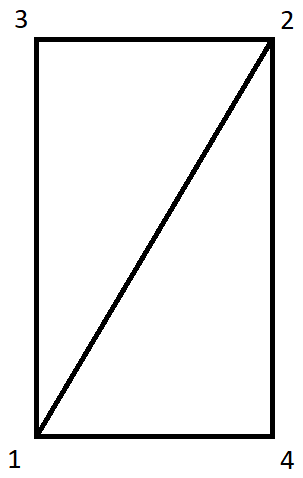
\includegraphics[width=0.25\textwidth]{kepek/billboardFrame.png}
 \label{fig:billboardFrame}
\end{wrapfigure}
A pontok meghatározását a calculateBillboardVertices() metódus végzi. A textúrán 4 sorban és 8 oszlopban helyezkednek el rajta az állapotok, tehát egy állapot oldalainak aránya 2:1. Ez azt jelenti hogy a megjelenítésnél egy téglalapra kell ráhúzni képeket. A téglalapot természetesen 2 háromszög alkotja, amint az a \ref{fig:billboardFrame}. ábrán is látszik. 
Mivel az alakzatot az Y tengely körül kell majd a későbbiekben forgatni, érdemes úgy definiálni a pontokat, hogy a téglalap alsó élének középpontja az origóba essen, hogy az a forgatás során egy helyben maradjon. A téglalap síkja pedig az XY síkkal esik majd egybe, mert így egyszerűbb definiálni. Konkrét koordinátákkal is meghatározhatnám a téglalapot, de akkor minden kirajzolás esetén a modellmátrixot a skála paraméternek megfelelően kell skálázni. Hogy ezt a műveletet megspóroljam, eleve a skála segítségével határozom meg a koordinátákat. Az Y koordináták a vagy a skála értékét veszik fel, az X koordináták azonban a $\pm \frac{\text{skála paraméter}}{4}$ értékeket, hiszen a magasság felét még az origó is kettéosztja. A pontokat az óramutató járásának irányával ellentétes sorrendben érdemes megadni, hogy a későbbiekben ha szükséges, könnyen lehessen belőlük normálvektort számítani. Így tehát az első háromszög pontjai az 1, 2, 3 pontok, a másodikéi pedig 1, 4, 2. A pontokat ebben a sorrendben kell tárolni, ehhez mindig a C++ standard könyvtárának vektor típusú tárolóját használom, ugyanis kezelése könnyű, dinamikus a mérete és felszabadítja a lefoglalt helyet maga után.

%calculateNextTextureCoordinates()
Az ezekhez a pontokhoz tartozó textúra koordinátákat a calculateNextTextureCoordinates() metódussal állítom elő. Mivel egy képen van több állapotom, ezek az értékek állapotról állapotra változnak. Egy adattag (m\_iActualFrame) segítségével számon tartom, hogy éppen hanyadik állapotnál járok, és ebből a számból határozom meg a hozzá tartozó koordinátákat. A számozást 0-tól kezdem. Először a sor és oszlopszámot kell kiszámolni hozzá. A sort az $\frac{\text{állapot sorszáma}}{\text{oszlopok száma}}$ hányados egész része adja meg, az oszlopot pedig az előbbi osztás maradéka (modulo művelet). A textúra koordináták a bal felső sarokból (0,0) indulnak, és a jobb alsó sarok (1,1) felé nőnek. Az adattagok között számon tartom, hogy egy állapot a textúra koordináta-rendszernek megfelelően milyen széles(m\_fColumnstep), és milyen magas(m\_fRowstep). Ennek megfelelően például az állapot bal felső pont $(u, v)$ koordinátája az $u=\text{adott oszlop} \cdot \text{szélesség}$, és $v=\text{adott sor} \cdot \text{magasság}$, a jobb alsó pedig az  $u=(\text{adott oszlop} + 1) \cdot \text{szélesség}$, és $v=(\text{adott sor} + 1) \cdot \text{magasság}$ alapján kapható meg. Az így kapott $(u, v)$ koordinátákat a téglalap objektum pontjainak megfelelő sorrendben kell megadni, azaz 1, 2, 3, 1, 4, 2, ahol például 1 a bal alsó, 2 a jobb felső ponthoz tartozó koordináták. A metódus utolsó lépéseként növeljük az állapot sorszámát tároló adatag értékét eggyel, ügyelve arra, hogy az utolsó állapotot követően nullázzuk.

%VAO generálás
Ezek után generálunk egy VAO-t és a két vektort, melyeket az előbbi funkciókkal állítottunk elő, külön-külön VBO-k segítségével tároljuk a VAO-ban. A két VBO között fontos különbség, hogy amíg a pontokat statikus objektumként tároljuk le, addig a textúra koordinátákat dinamikusként kell, ugyanis ennek a VBO-nak a tartalma fog változni az animáció során. Ezt a GL\_DYNAMIC\_DRAW paraméter segítségével jelezhetjük a grafikus processzornak, amely így ennek megfelelően allokálja a buffer számára a helyet, például a saját memóriája helyett akár a gép memóriáját is használhatja.
A VBO generálás a következőképpen néz ki:
\begin{lstlisting}
glGenBuffers(1, &m_iFireVBO);
glBindBuffer(GL_ARRAY_BUFFER, m_iFireVBO);
glBufferData(GL_ARRAY_BUFFER, 
	textureCoordinates.size() * sizeof(glm::vec2), 
	&textureCoordinates.front(), GL_DYNAMIC_DRAW);
glEnableVertexAttribArray(m_pFireShader->attrib("vertTexCoord"));
glVertexAttribPointer(m_pFireShader->attrib("vertTexCoord"), 2, 
	GL_FLOAT, GL_FALSE, 0, NULL);
\end{lstlisting}
A glGenBuffers generál egy VBO-t és az azonosítóját beírja a második paramétereként megadott helyre, melyet a glBindBuffer-nek átadva ``használatba helyezhetjük'' (bind-eljük) a buffert. A glBufferData függvénnyel definiálhatjuk a buffer tartalmát, jelen esetben a textúra koordinátákat tároljuk majd benne. Az első paramétere megadja a buffer fajtáját, jelen esetben pontok tulajdonságára utaló adatokkal lesz feltöltve. A második paraméter a tároló objektum méretét adja meg, a harmadik pedig a címét. Az utolsó paraméter a VBO használatára utal. A példában GL\_DYNAMIC\_DRAW mellett még a GL\_STATIC\_DRAW konstanst használtam még az olyan aVBO-k esetén, melyek tartalmát nem változtatom. A glEnableVertexAttribArray függvény engedélyezi a megadott attribútum használatát a shader programban, a glVertexAttribPointer pedig megadja, hogy az adott VBO-t melyik attribútomon keresztül kapja meg a shader. Utóbbi függvény második paramétere adja meg, hogy hány komponensből áll egy csúcspont tulajdonság, ezt követi a komponensek típusa. A negyedik paraméter megadja, hogy az egész értékű adattípusokat normalizálja-e, vagy sem. Az utolsó előtti paraméter adja meg a pont tulajdonságok közti offset-et, végül pedig a bufferben az első tulajdonság előtti offset-et adjuk meg.

A loadVAO metódus tehát betöltött minden szükséges adatot, amely a kirajzoláshoz szükséges.

% DRAW
A kirajzolást a drawFire metódus végzi. Először be kell állítani a használni kívánt shader-t, majd bind-elni kell a használni kívánt textúrát. Ezt át is kell adni a shader-nek, esetemben a tex uniform-on keresztül. Ezt követően bind-eljük a VAO-t, amelyben a pontok adatait tároljuk. Az átlátszóság kezelése miatt a mélység puffer írását kikapcsoljuk a rajzolás idejére, ennek pontos okára a későbbiekben térek majd ki. Ha csupán egy billboardot szeretnénk kirajzolni, akkor megadjuk a shader-nek a modell mátrixot (amely az eltolást és az esetleges forgatást végzi el a pontokon), majd a glDrawArrays segítségével kirajzoljuk a háromszögeket. Ha szeretnénk 90 fokkal elforgatva is kirajzolni a billboardot, akkor a modell mátrixot még 90 fokkal elforgatjuk a GLM könyvtár rotate metódusának segítségével, ezt ismét átadjuk a shader-nek, eztán pedig megint kirajzoljuk a VAO-t. Az átlátszóság kezelése miatt itt már a sorrendre is figyelni kell, de ezt is a későbbiekben fejtem majd ki. A rajzolások után engedélyezzük a méylség puffer írását, kikapcsoljuk az adott VAO, textúra és shader használatát. A drawFire metódus végén az m\_fElapsedTime adattaghoz hozzáadjuk az előző kirajzolás óta eltelt időt, melyet a camera onjektumtól kérdezhetünk le. Ebben az adattagban számoljuk az előző állapotváltás óta eltelt időt. Amennyiben ez átlépi a határt (m\_fAnimationSpeed), a következő állapot textúra koordinátáit kell betöltenünk. Ehhez bind-elni kell az adott VBO-t, majd a calculateNextTextureCoordinates metódus segítségével előállítani a megfelelő textúra koordinátákat. A buffer tartalmát a glBufferSubData függvény segítségével írhatjuk át. Ezzel a buffer tartalmának egy részét is át lehetne írni, de nekem az egészet át kell. Ennek ellenére is hatásosabb ezt használni a glBufferData helyett, ugyani így a szükséges memória újraallokálását el lehet kerülni. Végül nullázzuk az m\_fElapsedTime adattagot.

% shaderek
A vertex és fragmet shaderek itt rendkívül egyszerűek. A vertex shader csak a csúcspontokat és a textúra koordinátákat kapja meg a szükséges transzformációs mátrixok mellett. A pontokat továbbadja a fragment shader-nek, a pozíciót (gl\_Position) pedig a kamera és modell mátrixokkal megszorzott homogén koordinátával kibővített (TODO: helyes ez így?) csúcspont helye adja meg. A fragment shader pedig a uniform-ként kapott textúrából a textúra koordináta alapján kiolvasott értéket adja meg a pixel színeként. 

%Sprite osztály
\subsection{SpriteFire osztály}
A sprite tűzhöz külön osztályt készítettem. A SpriteFire osztály egyik adattagja BillboardFire típusú, hiszen abban már implementálva van az egyszerű 1 téglalapon alapuló megjelenítés is. A SpriteFire konstruktorának szüksége van a tűzhöz használt shader program, a camera objektum és a tűz megjelenítési pozíciójára is. A skála paraméter itt is opcionális. Ezen paraméterek segítségével inícializálom a BillboardFire adattagot úgy, hogy csak egy felületet rajzoljon ki. A drawFire metódus itt csak beállítja a BillboardFire adattag elfordulását a setRotation metódusával, majd meghívja annak a drawFire metódusát. Az elfordulást a calculateRotation metódus állapítja meg:
\begin{lstlisting}
float angle = 0.f;
glm::vec2 cameraPos(m_pCamera->getX(), m_pCamera->getZ());
glm::vec2 firePos(m_vPosition.x, m_vPosition.z);

glm::vec2 eye = glm::normalize(cameraPos - firePos);

float cosAlpha = glm::dot(eye, glm::vec2(0.f, -1.f)); 

if (cameraPos.x < firePos.x)
{
	angle = glm::acos(cosAlpha);
}
else
{
	angle = glm::acos(-cosAlpha);
}

return angle;
\end{lstlisting}
Mivel a tűz alap esetben a -Z tengely felé néz, ehhez a tengelyhez kell mérni az elfordulást is. Ehhez szükség van a kamera és a tűz XZ sík menti pozícióira (cameraPos, firePos). Az eye vektor a tűz pozíciójából a kamera pozíciójába bocsátott vektor. Az $\bar{a}$ és $\bar{b}$ vektor által bezárt szög koszinuszát a következő egyenlet alapján kaphatjuk meg: 
\begin{center}
$\cos \alpha = \frac{\bar{a} \cdot \bar{b}}{|\bar{a}| \cdot |\bar{b}|}$
\end{center}
Amennyiben a két vektor normalizált, azaz a hosszuk egységnyi hosszú, az egyenletben az osztó értéke 1, tehát azt el is hagyhatjuk. Ezért a cosAlpha változó értékéhez elég a két vektor (eye és -Z) skaláris szorzatát venni. Mivel a két vektor által bezárt szög definíció szerint kisebb, vagy egyenlő, mint 180$^{\circ}$, a két pozíció X tengely menti helyzetéhez viszonyítva el kell dönteni, hogy mikor kell a szög -1-szeresével számolni. 

% átlátszóság, mélység puffer
\subsection{Az átlátszóság kezelése}

% fps, pontok száma, 
\subsection{Számításigény}

% Képek

\section{Háromdimenziós részecskerendszer alapú tűz}
















